\subsection{Khắc Phục Vi Phạm}
% -----------------------------------------------------------------------------

Năm phương pháp chính, từ đơn giản đến phức tạp. Lựa chọn dựa trên bản chất của dữ liệu và mục tiêu mô hình hóa.

\begin{center}
\begin{tabular}{@{}lp{5.2cm}l@{}}
\toprule
\textbf{Phương pháp} & \textbf{Phù hợp khi} & \textbf{Giữ nguyên OLS?} \\
\midrule
Biến đổi biến số    & Quan hệ mũ hoặc lũy thừa đơn giản         & Có, sau biến đổi \\
Hồi quy đa thức     & Quan hệ cong vừa phải, toàn vùng           & Có \\
Splines             & Độ cong cục bộ; tránh méo biên              & Có \\
Hồi quy phi tuyến  & Dạng hàm có cơ sở lý thuyết rõ ràng        & Không---cần lặp số \\
GLMs                & Biến phản hồi bị chặn hoặc là số đếm       & Không---dùng hàm liên kết \\
\bottomrule
\end{tabular}
\end{center}

% - - - - - - - - - - - - - - - - - - - - - - - - - - - - - - - - - - - - - -
\subsubsection{Biến Đổi Biến Số}

Thay thế $X$, $Y$, hoặc cả hai bằng một biến đổi làm thẳng quan hệ trước khi khớp OLS.

\begin{center}
\begin{tabular}{@{}lll@{}}
\toprule
\textbf{Dạng quan hệ thực} & \textbf{Biến đổi gợi ý} & \textbf{Mô hình sau biến đổi} \\
\midrule
$Y = \beta_0 \cdot e^{\beta_1 X}$ & $\log(Y)$ & $\log(Y) = \gamma_0 + \gamma_1 X$ \\
$Y = \beta_0 \cdot X^{\beta_1}$   & $\log(Y)$ và $\log(X)$ & $\log(Y) = \gamma_0 + \gamma_1\log(X)$ \\
$Y = \beta_0 / (\beta_1 + X)$     & $1/Y$ hoặc $1/X$ & (tùy trường hợp) \\
\bottomrule
\end{tabular}
\end{center}

Khi không rõ nên dùng biến đổi nào, \textbf{phương pháp Box-Cox} tìm kiếm $\lambda$ tối ưu hóa hàm log-likelihood:
\[
  y^{(\lambda)} = \begin{cases} (y^\lambda - 1)/\lambda & \lambda \neq 0 \\ \log y & \lambda = 0 \end{cases}
\]
$\lambda = 0$ tương ứng biến đổi log; $\lambda = 0.5$ tương ứng căn bậc hai. Khoảng tin cậy 95\% cho $\lambda$ từ profile likelihood chỉ ra biến đổi phù hợp.

\begin{figure}[H]
  \centering
  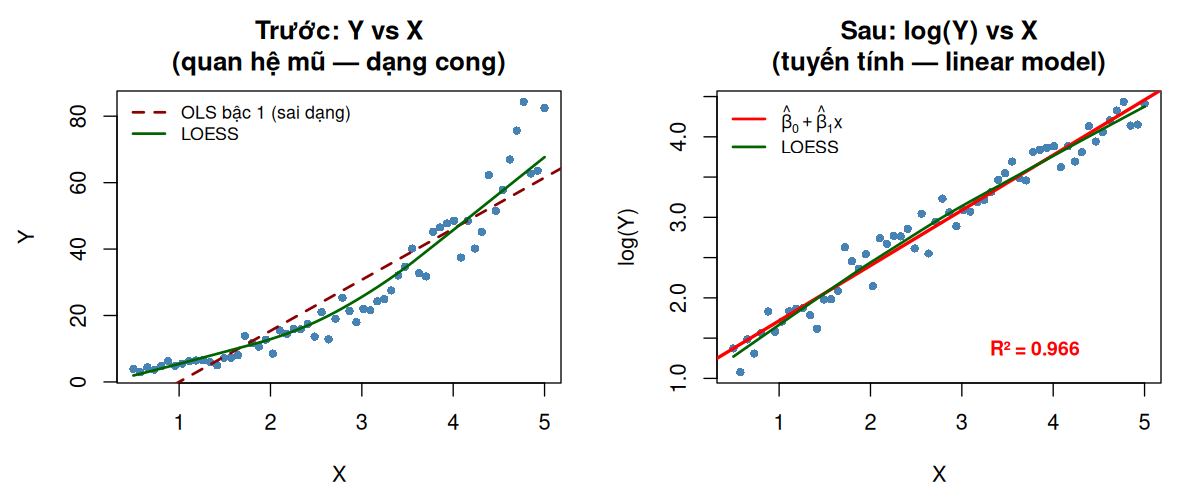
\includegraphics[width=0.9\textwidth]{./figures/fig4_log_transform.png}
  \caption{Biến đổi $\log(Y)$ tuyến tính hóa quan hệ mũ.
  Trái: $Y$ theo $X$ dạng cong, OLS bậc 1 bỏ lỡ xu hướng.
  Phải: $\log(Y)$ theo $X$ quan hệ tuyến tính, OLS và LOESS trùng khớp.
  Hệ số $\gamma_1$ diễn giải trực tiếp là phần trăm thay đổi của $Y$ khi $X$ tăng 1 đơn vị.}
  \label{fig:log_transform}
\end{figure}

\begin{lstlisting}[style=Rstyle]
library(MASS)
# Box-Cox: tim lambda toi uu
bc <- boxcox(mpg ~ hp + wt, data = mtcars)
lambda_opt <- bc$x[which.max(bc$y)]
cat("lambda toi uu:", round(lambda_opt, 2), "\n")
# lambda ~ 0 -> dung log(Y); lambda ~ 0.5 -> dung sqrt(Y)
\end{lstlisting}

% - - - - - - - - - - - - - - - - - - - - - - - - - - - - - - - - - - - - - -
\subsubsection{Hồi Quy Đa Thức}

Bổ sung lũy thừa nguyên của biến dự báo làm biến hồi quy. Đây vẫn là \textbf{mô hình tuyến tính} vì tuyến tính trong $\beta$.

\paragraph{Một biến dự báo.}
\[
  E(Y \mid X = x) = \beta_0 + \beta_1 x + \beta_2 x^2 + \cdots + \beta_d x^d
\]

\paragraph{Nhiều biến dự báo.}
Mô hình bậc hai với $X_1$ và $X_2$ thêm cả tương tác:
\[
  E(Y \mid x_1, x_2) = \beta_0 + \beta_1 x_1 + \beta_2 x_2
                      + \beta_{11} x_1^2 + \beta_{22} x_2^2 + \beta_{12} x_1 x_2
\]

Tổng quát với $k$ biến: $1 + k + k + k(k-1)/2$ tham số cho mô hình bậc hai.

\paragraph{Ứng dụng nổi bật: xác định cực trị.}
Khi $d = 2$, đỉnh hoặc đáy của parabol xảy ra tại:
\[
  x_M = -\frac{\beta_1}{2\beta_2}
\]
Hữu ích trong tối ưu hóa (liều thuốc tối ưu, nhiệt độ vận hành tốt nhất, \ldots).

\paragraph{Rủi ro chính.}
Đa thức là hàm \textit{toàn cục}: bậc cao khớp tốt ở giữa nhưng dao động mạnh ở biên (xem hình~\ref{fig:splines}). Dùng \texttt{poly(X, d)} thay vì \texttt{I(X\^{}2)} để nhận đa thức trực giao, tránh đa cộng tuyến số.

% - - - - - - - - - - - - - - - - - - - - - - - - - - - - - - - - - - - - - -
\subsubsection{Splines}

Splines chia phạm vi $X$ thành các đoạn tại các \textbf{nút} (knots) và khớp một đa thức bậc thấp riêng biệt trong từng đoạn, nối trơn tại ranh giới. Khác với đa thức toàn cục, splines là \textit{cục bộ}: độ cong ở một vùng không làm méo dự báo ở vùng khác.

Cubic B-splines là cơ sở tiêu chuẩn: mỗi hàm cơ sở khác không chỉ trên một khoảng nhỏ, đảm bảo đường cong trơn đến đạo hàm bậc hai tại mọi nút và tính toán ổn định về số.

\begin{figure}[H]
  \centering
  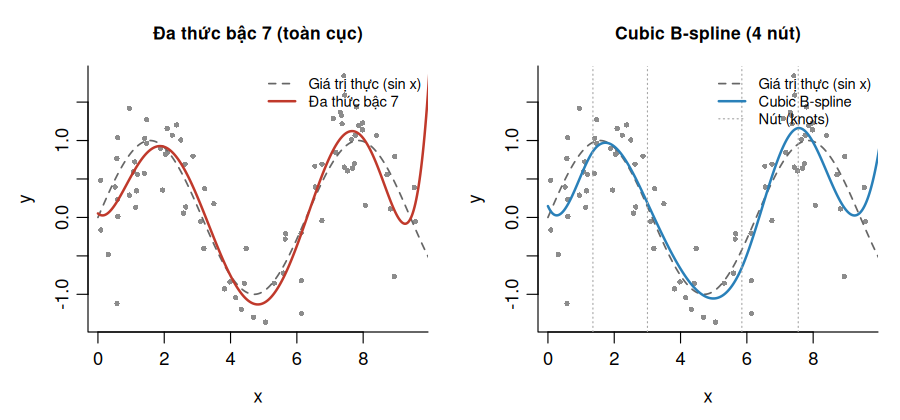
\includegraphics[width=\textwidth]{./figures/fig9_splines.png}
  \caption{Đa thức bậc 7 (toàn cục) so với cubic B-spline với 4 nút trên dữ liệu $y = \sin(x) + \varepsilon$.
  \textbf{Trái:} Đa thức bậc 7 khớp tốt ở giữa nhưng dao động mạnh ở biên trái và phải, lệch xa giá trị thực.
  \textbf{Phải:} Cubic B-spline bám sát $\sin(x)$ ổn định trên toàn vùng; các đường đứt nét thẳng đứng là vị trí nút.}
  \label{fig:splines}
\end{figure}

\begin{lstlisting}[style=Rstyle]
library(splines)
# Cubic B-spline voi nut tai phan vi 25, 50, 75
fit_spl <- lm(mpg ~ bs(hp,
                       knots  = quantile(mtcars$hp, c(0.25, 0.5, 0.75)),
                       degree = 3),
              data = mtcars)

hp_seq  <- seq(min(mtcars$hp), max(mtcars$hp), length.out = 300)
pred_sp <- predict(fit_spl, newdata = data.frame(hp = hp_seq))

plot(mtcars$hp, mtcars$mpg, pch = 16, col = "gray50",
     xlab = "hp", ylab = "mpg")
lines(hp_seq, pred_sp, col = "blue", lwd = 2)
\end{lstlisting}

% - - - - - - - - - - - - - - - - - - - - - - - - - - - - - - - - - - - - - -
\subsubsection{Hồi Quy Phi Tuyến}

Khi quan hệ được chi phối bởi một cơ chế lý thuyết đã biết---suy giảm mũ, tăng trưởng logistic, động học Michaelis-Menten---khớp mô hình với tham số tương tác \textit{phi tuyến}:
\[
  y = \beta_0 + \beta_1 \exp(\beta_2 x) + \varepsilon
\]

Nghiệm dạng đóng OLS không áp dụng. Tham số được ước lượng lặp bằng \textbf{thuật toán Gauss-Newton}: tuyến tính hóa mô hình quanh ước lượng hiện tại, cập nhật tham số, lặp lại cho đến hội tụ. Cần cung cấp giá trị khởi đầu hợp lý; nếu không, thuật toán có thể không hội tụ hoặc hội tụ về cực tiểu cục bộ.

\textbf{Khi nào nên dùng:} chỉ khi có dạng hàm có cơ sở lý thuyết. Nếu chỉ cần khớp đường cong mà không có cơ chế cụ thể, splines thường ưu tiên hơn.

\begin{lstlisting}[style=Rstyle]
# Hoi quy phi tuyen: Y = a * exp(b * X) + c
# nls() yeu cau gia tri khoi dau
fit_nls <- nls(mpg ~ a * exp(b * hp) + c,
               data  = mtcars,
               start = list(a = 50, b = -0.005, c = 5))
summary(fit_nls)$coefficients
\end{lstlisting}

% - - - - - - - - - - - - - - - - - - - - - - - - - - - - - - - - - - - - - -
\subsubsection{Mô Hình Tuyến Tính Tổng Quát (GLMs)}

Khi biến phản hồi có ràng buộc cấu trúc tự nhiên---xác suất bị chặn trong $[0,1]$, số đếm không thể âm---không có biến đổi nào của $X$ tạo được quan hệ đường thẳng với biến phản hồi bị chặn. GLMs giải quyết bằng \textbf{hàm liên kết} $g(\cdot)$:
\[
  g\!\left(E[Y \mid X]\right) = X\beta
\]

Tham số vẫn tuyến tính trong $X\beta$; hàm liên kết xử lý ánh xạ phi tuyến giữa thang biến phản hồi và không gian dự báo tuyến tính. Ước lượng bằng Maximum Likelihood, không phải OLS.

\begin{center}
\begin{tabular}{@{}llll@{}}
\toprule
\textbf{Kiểu phản hồi} & \textbf{Mô hình} & \textbf{Hàm liên kết} & \textbf{R} \\
\midrule
Nhị phân $\{0, 1\}$         & Logistic  & $\log\!\left(\frac{\mu}{1-\mu}\right)$ & \texttt{glm(..., binomial)} \\
Số đếm $\{0, 1, 2, \ldots\}$ & Poisson   & $\log(\mu)$ & \texttt{glm(..., poisson)} \\
Tỷ lệ $(0, 1)$              & Beta      & logit & \texttt{betareg()} \\
\bottomrule
\end{tabular}
\end{center}

% - - - - - - - - - - - - - - - - - - - - - - - - - - - - - - - - - - - - - -
\subsubsection{So Sánh Mô Hình}

Sau khi đề xuất các mô hình khác nhau, cần tiêu chí khách quan để chọn độ phức tạp phù hợp.

\textbf{ANOVA (kiểm định F cho mô hình lồng nhau):}
\[
  H_0{:}\ \text{Mô hình đơn giản hơn là đủ (hệ số bậc cao} = 0\text{)}
\]

Chỉ áp dụng cho mô hình lồng nhau. $p < 0.05$: mô hình phức tạp hơn cải thiện đáng kể.

\textbf{AIC và BIC:}
\[
  \text{AIC} = -2\log(L) + 2k
  \qquad
  \text{BIC} = -2\log(L) + k\log(n)
\]

Áp dụng được cho mô hình không lồng nhau. $\Delta\text{AIC} > 2$ đã có ý nghĩa; BIC phạt nặng hơn cho số tham số, ưu tiên mô hình đơn giản hơn.

\begin{center}
\small
\begin{tabularx}{\textwidth}{@{}l>{\raggedright\arraybackslash}X>{\raggedright\arraybackslash}X@{}}
\toprule
\textbf{Tiêu chí} & \textbf{Ưu điểm} & \textbf{Hạn chế} \\
\midrule
ANOVA & Kiểm định chính xác, $p$-value rõ ràng & Chỉ cho mô hình lồng nhau \\
AIC   & Linh hoạt, tốt cho dự báo              & Có thể chọn mô hình quá phức tạp \\
BIC   & Phạt nặng hơn, ưu tiên mô hình gọn     & Đôi khi quá thận trọng \\
\bottomrule
\end{tabularx}
\end{center}

\textbf{Cảnh báo quá khớp.} Bậc đa thức hoặc số nút spline quá cao thường dẫn đến quá khớp. Ưu tiên mô hình đơn giản nhất mà vẫn giải thích được xu hướng chính; kiểm tra đồ thị phần dư sau khi chọn mô hình.

% -----------------------------------------------------------------------------
\subsubsection{Đánh Giá Mô Hình Sau Khi Khắc Phục}
% -----------------------------------------------------------------------------

Sau khi áp dụng biến đổi, thêm số hạng đa thức, hoặc dùng spline, cần xác minh rằng mô hình mới thực sự cải thiện. Dưới đây là năm công cụ đánh giá thường dùng.

\begin{enumerate}

  \item \textbf{Đồ thị phần dư — kiểm tra trực quan đầu tiên.}
  Vẽ lại đồ thị phần dư theo giá trị khớp. Nếu phi tuyến đã được giải quyết, đồ thị trở thành ``null plot'': phân tán ngẫu nhiên, đường LOESS nằm ngang gần $y=0$. Đồng thời kiểm tra xem việc sửa chữa có làm lộ ra vi phạm khác (phương sai không đồng đều, điểm ngoại lai) hay không.

  \item \textbf{Adjusted $R^2$ — trừng phạt độ phức tạp.}
  Khi thêm số hạng mới, $R^2$ thông thường luôn tăng (dù số hạng đó vô nghĩa). Adjusted $R^2$ hiệu chỉnh theo bậc tự do:
  \[
    \bar{R}^2 = 1 - \frac{(1-R^2)(n-1)}{n-k-1},
  \]
  trong đó $k$ là số biến dự báo. Nếu thêm bậc mà $\bar{R}^2$ giảm hoặc không đổi, số hạng đó không đóng góp thực sự.

  \item \textbf{AIC và BIC — cân bằng độ khớp và độ phức tạp.}
  AIC và BIC đã trình bày ở trên. Chênh lệch $\Delta\text{AIC} > 2$ được coi là có ý nghĩa; BIC phạt nặng hơn nên ưu tiên mô hình gọn hơn khi cỡ mẫu lớn.

  \item \textbf{Cross-validation — đánh giá khả năng dự báo thực sự.}
  Chia dữ liệu thành tập huấn luyện và tập kiểm tra; ước lượng tham số trên tập huấn luyện rồi đo sai số dự báo trên tập kiểm tra. $k$-fold CV (thường $k=5$ hoặc $10$) là lựa chọn phổ biến.

  \item \textbf{PRESS (Prediction Sum of Squares) — leave-one-out.}
  PRESS tính tổng bình phương sai số dự báo khi lần lượt loại từng quan sát:
  \[
    \text{PRESS} = \sum_{i=1}^n \left(\frac{e_i}{1 - h_{ii}}\right)^2,
  \]
  với $h_{ii}$ là đòn bẩy (leverage) của quan sát $i$. Công thức này không yêu cầu fit lại mô hình $n$ lần. Mô hình có PRESS nhỏ hơn dự báo tốt hơn trên dữ liệu mới.

\end{enumerate}

\medskip
\noindent\textbf{Minh họa trực quan: trước và sau khi sửa.}
Hình~\ref{fig:model_eval} so sánh mô hình tuyến tính (hàng trên) và đa thức bậc 2 (hàng dưới) trên bộ dữ liệu \texttt{mtcars} với biến phản hồi \texttt{mpg} và biến dự báo \texttt{hp}. Đồ thị phần dư ở cột giữa là tín hiệu rõ nhất: đường LOESS cong hình chữ U (mô hình tuyến tính) biến thành đường nằm ngang gần $y=0$ (mô hình bậc 2).

\begin{figure}[H]
  \centering
  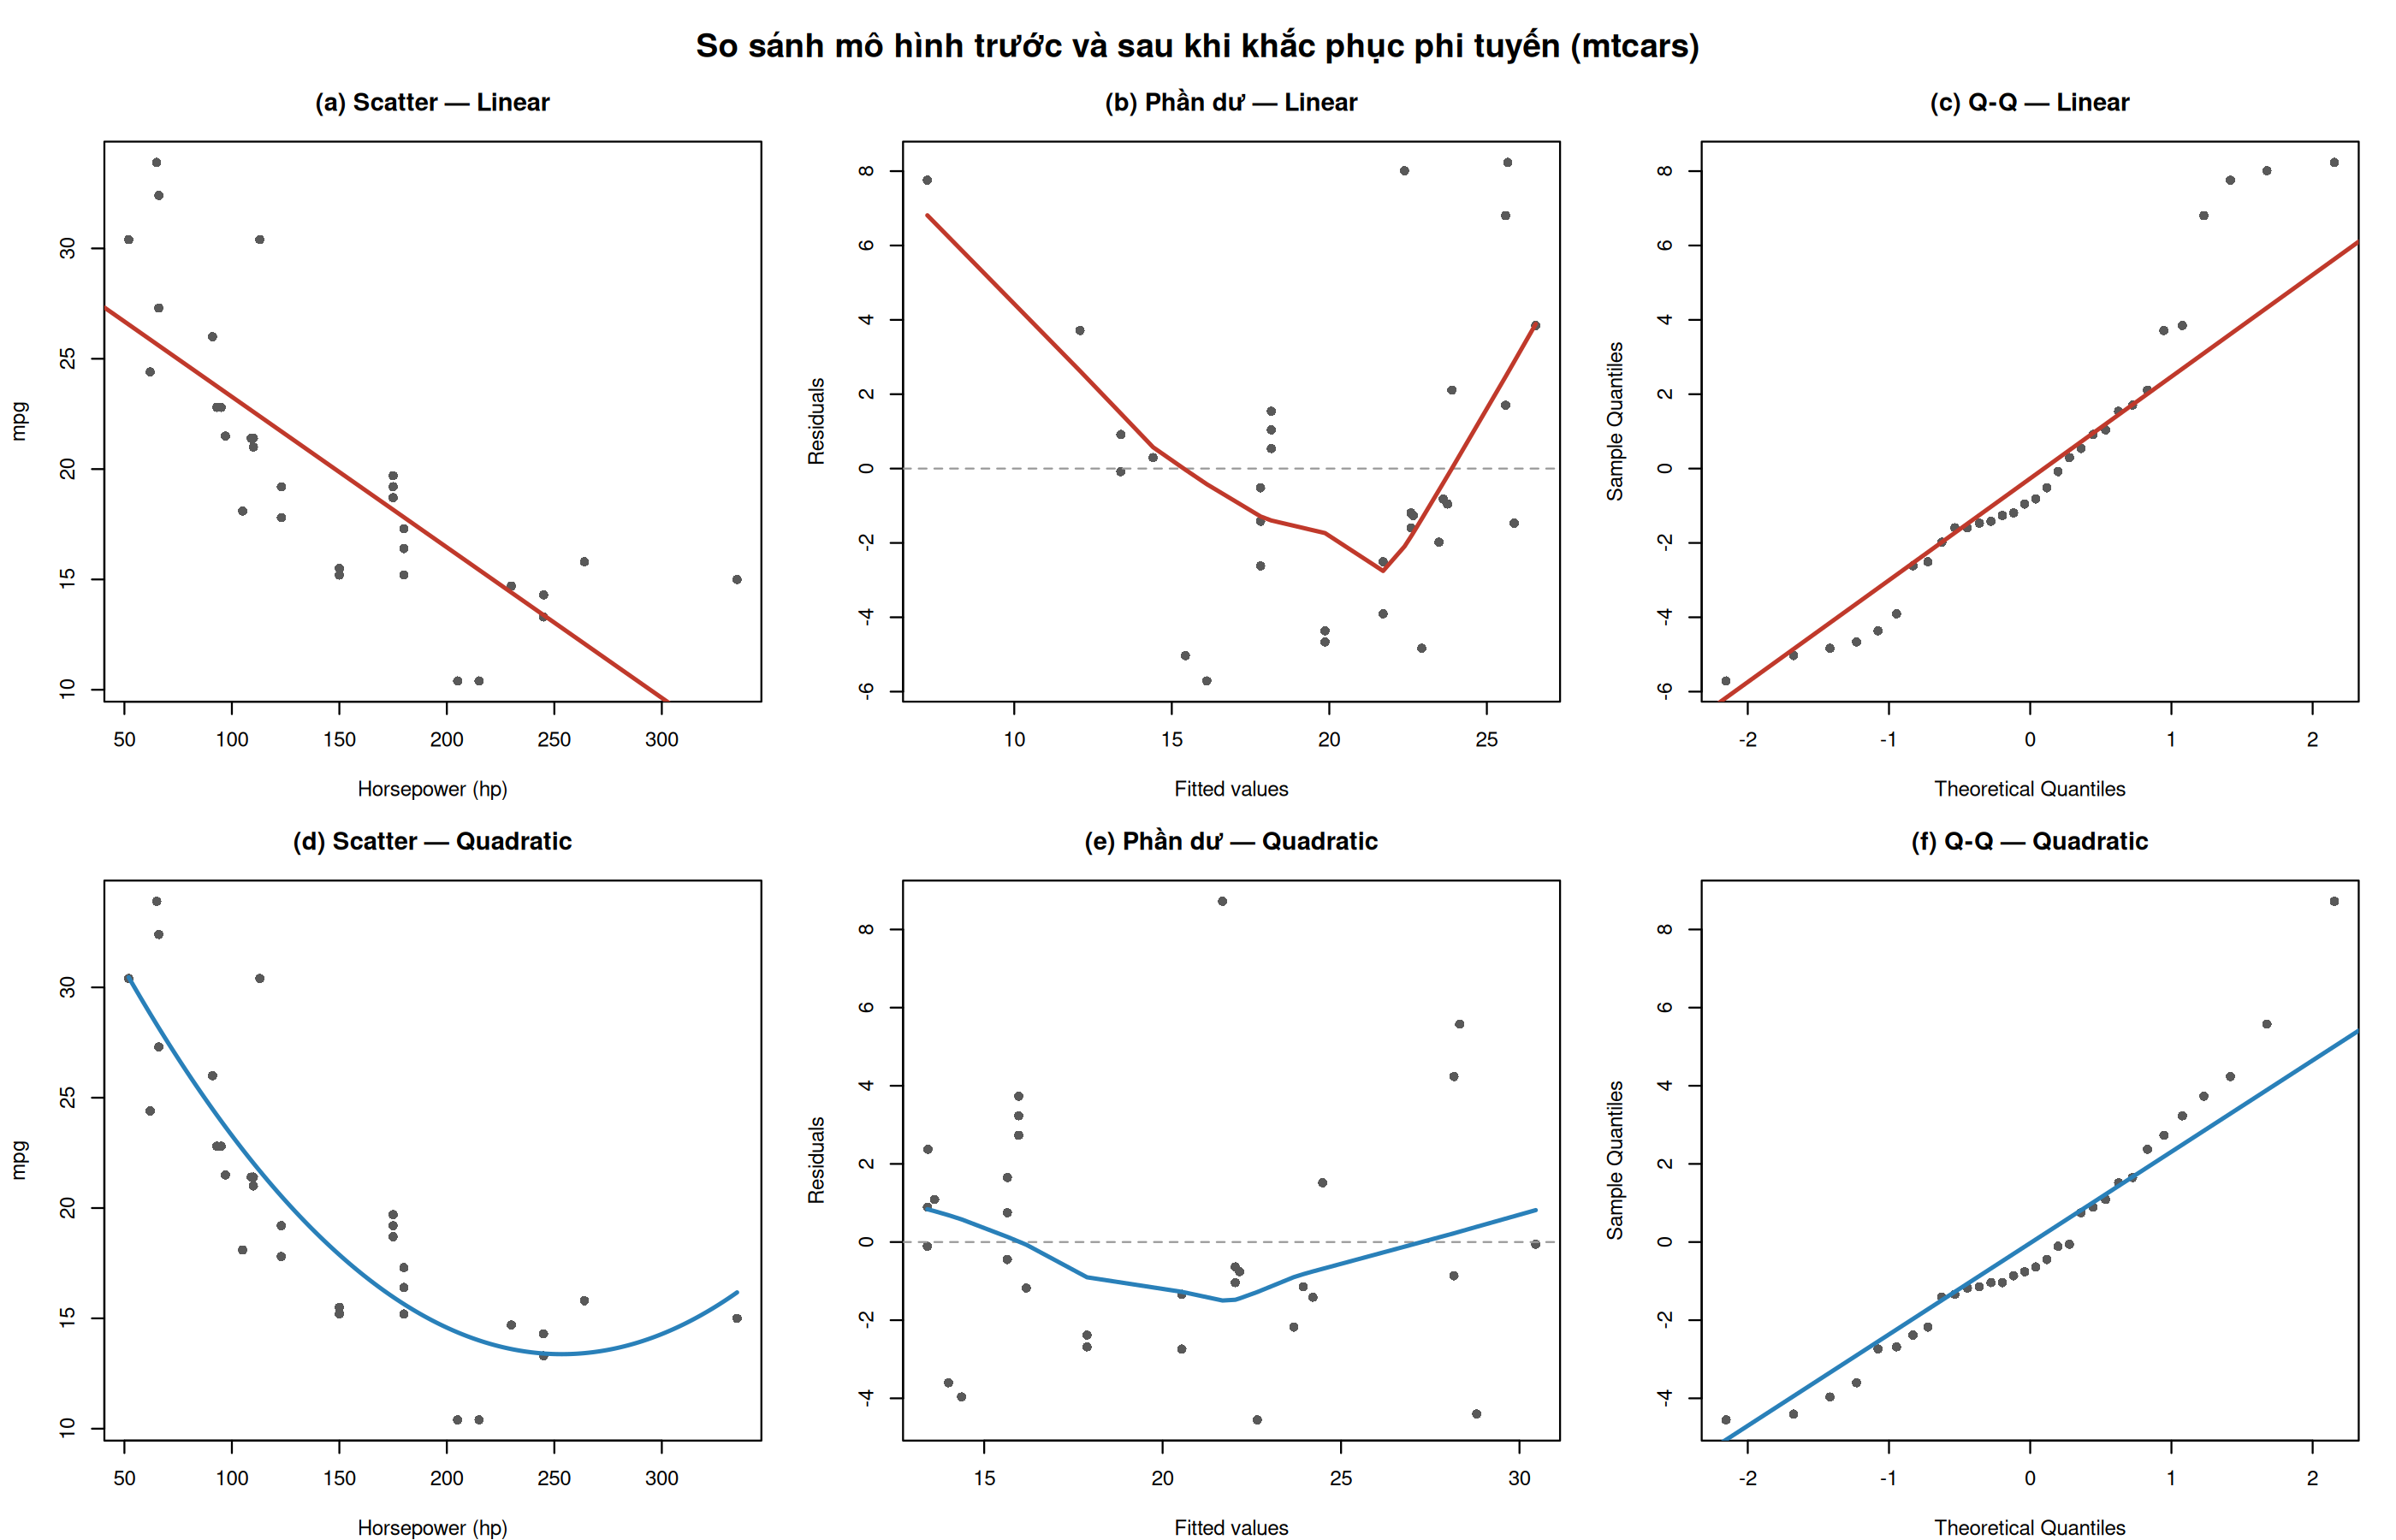
\includegraphics[width=\linewidth]{./figures/fig15_model_eval.png}
  \caption{So sánh mô hình tuyến tính (hàng trên) và đa thức bậc 2 (hàng dưới) trên \texttt{mtcars}. Cột trái: scatter và đường fit; cột giữa: phần dư theo giá trị khớp; cột phải: Q-Q plot. Đường LOESS hình chữ U trong panel (b) biến mất ở panel (e), xác nhận phi tuyến đã được khắc phục.}
  \label{fig:model_eval}
\end{figure}

\noindent\textbf{Bảng tổng hợp chỉ số đánh giá} (dataset \texttt{mtcars}, $n = 32$):

\begin{center}
\begin{tabular}{@{}lrrr@{}}
\toprule
\textbf{Chỉ số} & \textbf{Linear} & \textbf{Quadratic} & \textbf{Cubic} \\
\midrule
$R^2$                 & 0.602 & 0.756 & 0.761 \\
Adj.\ $R^2$           & 0.589 & 0.739 & 0.735 \\
AIC                   & 181.2 & 167.6 & 169.0 \\
BIC                   & 185.6 & 173.5 & 176.3 \\
PRESS                 & 552.1 & 338.0 & 338.4 \\
\bottomrule
\end{tabular}
\end{center}

\textbf{Diễn giải bảng.} Mô hình bậc 2 cải thiện đáng kể so với tuyến tính: Adj.\ $R^2$ tăng từ 0.589 lên 0.739, AIC giảm $\approx 13.6$ đơn vị, PRESS giảm từ 552 xuống 338 (giảm 39\%). Mô hình bậc 3 không cải thiện thêm (Adj.\ $R^2$ giảm, AIC tăng nhẹ, PRESS gần như bằng nhau) — bằng chứng quá khớp tiềm năng. Mô hình bậc 2 là lựa chọn tốt nhất theo cả năm tiêu chí.

\begin{lstlisting}[style=Rstyle]
data(mtcars)
model_lin  <- lm(mpg ~ hp,          data = mtcars)
model_quad <- lm(mpg ~ poly(hp, 2), data = mtcars)
model_cub  <- lm(mpg ~ poly(hp, 3), data = mtcars)

# Adj R2
sapply(list(model_lin, model_quad, model_cub),
       function(m) round(summary(m)$adj.r.squared, 3))

# AIC / BIC
AIC(model_lin, model_quad, model_cub)
BIC(model_lin, model_quad, model_cub)

# PRESS (leave-one-out, khong can fit lai n lan)
press <- function(fit) sum((residuals(fit) / (1 - hatvalues(fit)))^2)
sapply(list(model_lin, model_quad, model_cub), press)
\end{lstlisting}

% -----------------------------------------------------------------------------
